\clearpage
\newpage

\subsubsection{Estensione C: Modifica Rapida dello Stato delle Notifiche dalla Barra Laterale}

Per migliorare l’accessibilità e rendere la gestione delle notifiche più immediata, il sistema offre un metodo alternativo per attivare e disattivare le notifiche direttamente dalla barra laterale. Questa estensione elimina la necessità di accedere alla schermata dedicata, offrendo un controllo contestuale più rapido ed efficace.

\vspace{0.5cm}
\subsubsection{Interfaccia e Interazione}
Ogni categoria di notifica presente nella barra laterale include un pulsante contestuale che consente di modificarne lo stato. Il pulsante ha due possibili stati:

\begin{itemize}
    \item \textbf{Attiva}, se la categoria è attualmente disabilitata.
    \item \textbf{Disattiva}, se la categoria è attualmente abilitata.
\end{itemize}

Quando l’utente interagisce con il pulsante:
\begin{itemize}
    \item Se clicca su \textbf{Disattiva}, appare un popup di conferma che informa sulle implicazioni della disattivazione, in linea con i principi di prevenzione degli errori di Nielsen \cite{nielsen1995}.
    \item Se l’utente conferma, il sistema esegue una transizione animata per spostare la categoria dalla sezione delle notifiche attive a quella delle notifiche disattivate.
    \item Il pulsante cambia stato, diventando \textbf{Attiva}, in modo da riflettere visivamente la modifica e garantire un feedback immediato.
\end{itemize}

\subsubsection{Feedback Visivo e UX Design}
Per rendere il cambiamento chiaro e intuitivo, il sistema implementa le seguenti tecniche di UX design:
\begin{itemize}
    \item \textbf{Popup di conferma}: viene visualizzato prima di procedere con la modifica, seguendo le euristiche di usabilità per la prevenzione degli errori \cite{nielsen1995}.
    \item \textbf{Animazione di transizione}: la categoria viene spostata visivamente tra le sezioni della barra laterale, applicando il principio della \textbf{gestalt della continuità} \cite{miller1956} per rendere il cambiamento più naturale.
    \item \textbf{Aggiornamento dello stato del pulsante}: il pulsante cambia dinamicamente per riflettere lo stato attuale della categoria, riducendo l’ambiguità e migliorando la prevedibilità dell’interazione.
\end{itemize}

Questa estensione garantisce un’esperienza utente più fluida e immediata, riducendo il numero di passaggi necessari per la gestione delle notifiche senza compromettere la chiarezza e il controllo dell’utente.


\begin{figure}[ht]
    \centering
    \begin{tikzpicture}[node distance=1.5cm and 1cm, auto]
        % Nodo per immagine 1 con didascalia sotto
        \node (img1) {
            \begin{tabular}{c}
                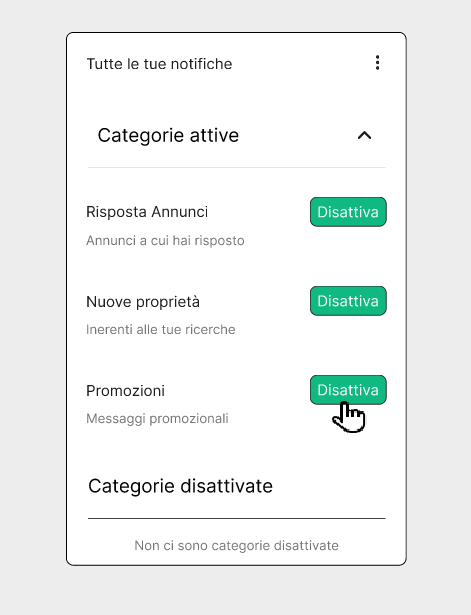
\includegraphics[width=0.4\textwidth]{Immagini/Mockup/notifiche/ESTENSIONE C/clickDisattiva.png} \\
                Cockburn: Extension C.2
            \end{tabular}
        };
        
        % Nodo per immagine 2 con didascalia sotto, posizionato a destra di img1
        \node (img2) [below=of img1] {
            \begin{tabular}{c}
                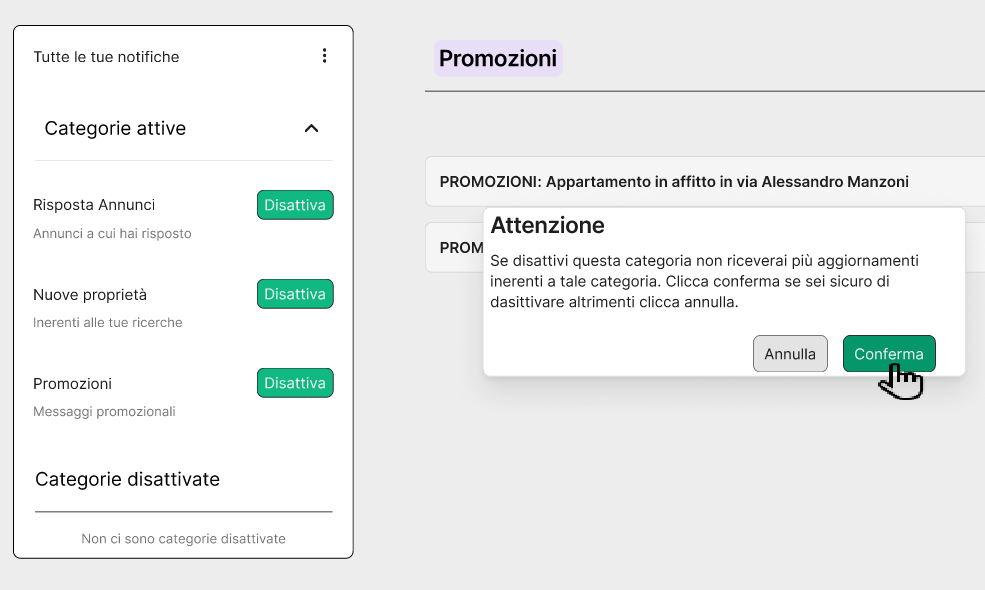
\includegraphics[width=.6\textwidth]{Immagini/Mockup/notifiche/ESTENSIONE C/clickCoonferma.png} \\
                Cockburn: step 6/7
            \end{tabular}
        };
        
        % Nodo per immagine 3 con didascalia sotto, posizionato sotto img2
        \node (img3) [below=of img2] {
            \begin{tabular}{c}
                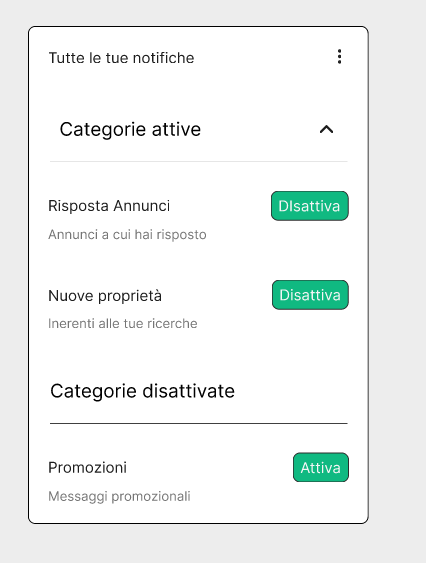
\includegraphics[width=0.3\textwidth]{Immagini/Mockup/notifiche/ESTENSIONE C/disattivato.png} \\
                Cockburn: step 8/9/10
            \end{tabular}
        };
        
        % Disegna le frecce
        \draw[->, thick] (img1) -- (img2);
        \draw[->, thick] (img2) -- (img3);
      
    \end{tikzpicture}
    \caption{Mockup: estensione C della tabella di Cockburn del caso d'uso disattiva/attiva categoria notifica}
    \label{fig:tikz_flow}
\end{figure}

\newpage

